\documentclass{article}
\usepackage{geometry}
\usepackage{graphicx}
\usepackage{titling}
\usepackage{url}

\title{Evaluation of RF technologies for Indoor Localization}
\author{Xuanjiao Zhu}
\date{\today}

\begin{document}

\begin{titlingpage}

\maketitle

\begin{abstract}
\textit{Location-based services} have become an important market recently, and the market is growing rapidly. These services are generally based on identifying the physical location of individuals or objects. although GPS is typically used outdoors, it is not suitable for indoor localization. Several alternatives have been developed over the years, including vision-based and radio frequency (RF)-based technologies. We report on our experiments with two RF technologies (ANT~\cite{ANT} and Bluetooth Low Energy~\cite{BT}) and their effectiveness in indoor environments.
\end{abstract}

\end{titlingpage}

\section{Introduction}
GPS(global positioning system), which uses signals of GPS satellites, is not a suitable solution of indoor localization. Instead, we are implementing a indoor localization system with two RF technologies: ANT and BLE. The system estimate the location of an object by using RSSI value. At the end, we discuss their performance in indoor localization.
\section{RF technologies}
There are varies of RF technologies. In this project we focus on two RF technologies: ANT and BLE.

\subsection{ANT}

ANT is a ultra low power wireless protocol. It is suited for multiple topologies: peer to peer, star, tree, mesh. It is a good solution for local area network(LAN). For example, smart home and automation Industries. ANT technology supports the use of any of the available 125 unique RF operating frequencies on 2.4Hz frequency band (2400MHz - 2524MHz)

\subsection{BLE}

BLE (Bluetooth Low Energy) is designed for low power network. It support peer to peer and broadcast, and mesh topologies. BLE operates on 2.4GHz frequency band. BLE uses frequency-hopping spread spectrum method. During the transmission, the radio signals switch among many frequency channel. The table shows a detailed comparison between ANT and BLE protocol on NRF module

\begin{table}[!h]
\begin{center}
\caption{ANT and BLE comoarison}
\label{ANT and BLE comoarison}
\begin{tabular}{|l|p{5cm}|p{5cm}|}
\hline
Description & BLE  &  ANT \\
\hline
Frequency range & 2.400--2.483 GHz &  2.00--2.483  \\
\hline
Frequency & FHSS &  Fixed frequency  \\
\hline
Supported topologies & Peer-to-peer,star & Peer-to-peer star ,mesh \\
\hline
Band & ISM 2.4GHz & ISM 2.4GHz \\
\hline
Security & 128-bit AES  & 64-bit key, 128 - bit AES \\
\hline 
Data rate &	2 Mbps, 1 Mbps, 500 kbps, 125 kbps	 & 1 Mbps \\
\hline
Number of connections	 & Up to 20	& Very high \\
\hline
Effective throughput	 & Up to 1.4 Mbps	& Up to 60 kbps \\
\hline
Applications	& Wearables, automation, sensors, fitness, healthcare, toys, computer peripherals, remote controls, etc.	 & Wireless sensors, hubs for sports, fitness, healthcare \\
\hline
\end{tabular}
\end{center}
\end{table}


\section{Methodology}

To localize an object,  first we need to get the distance between object and beacons. The distance can be estimated by RSSI. In this project, I implemented two platform, which is used to measure RSSI based on two RF technologies, ANT and BLE.

\subsection{ANT Setup}

This section introduces the way to set up a platform for measuring RSSI. Including setup in the host PC, base station and beacons.
	
\begin{figure}[!h]
\begin{center}
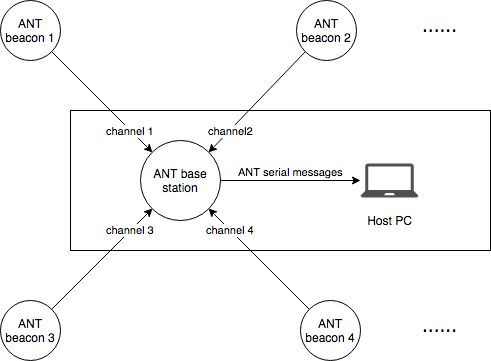
\includegraphics[width=0.5\columnwidth]{Figures/ANT_topology_laptop.jpg}
\caption{ANT Topology}
\label{ANT_topology}
\end{center}
\end{figure}

\subsubsection{ANT beacon} 
The ANT beacons are the masters which initiate communication. They are assigned to different frequency channel. The ANT beacon broadcasts  its serial number and its channel ID with designated channel period (Figure \ref{ANT_base_station_listening}). In this project, ANT beacons are ANT SoC  "D52QD2M6IA-A" (shown in figure \ref{ANT_layers}) .

\begin{figure}[!h]
\begin{center}
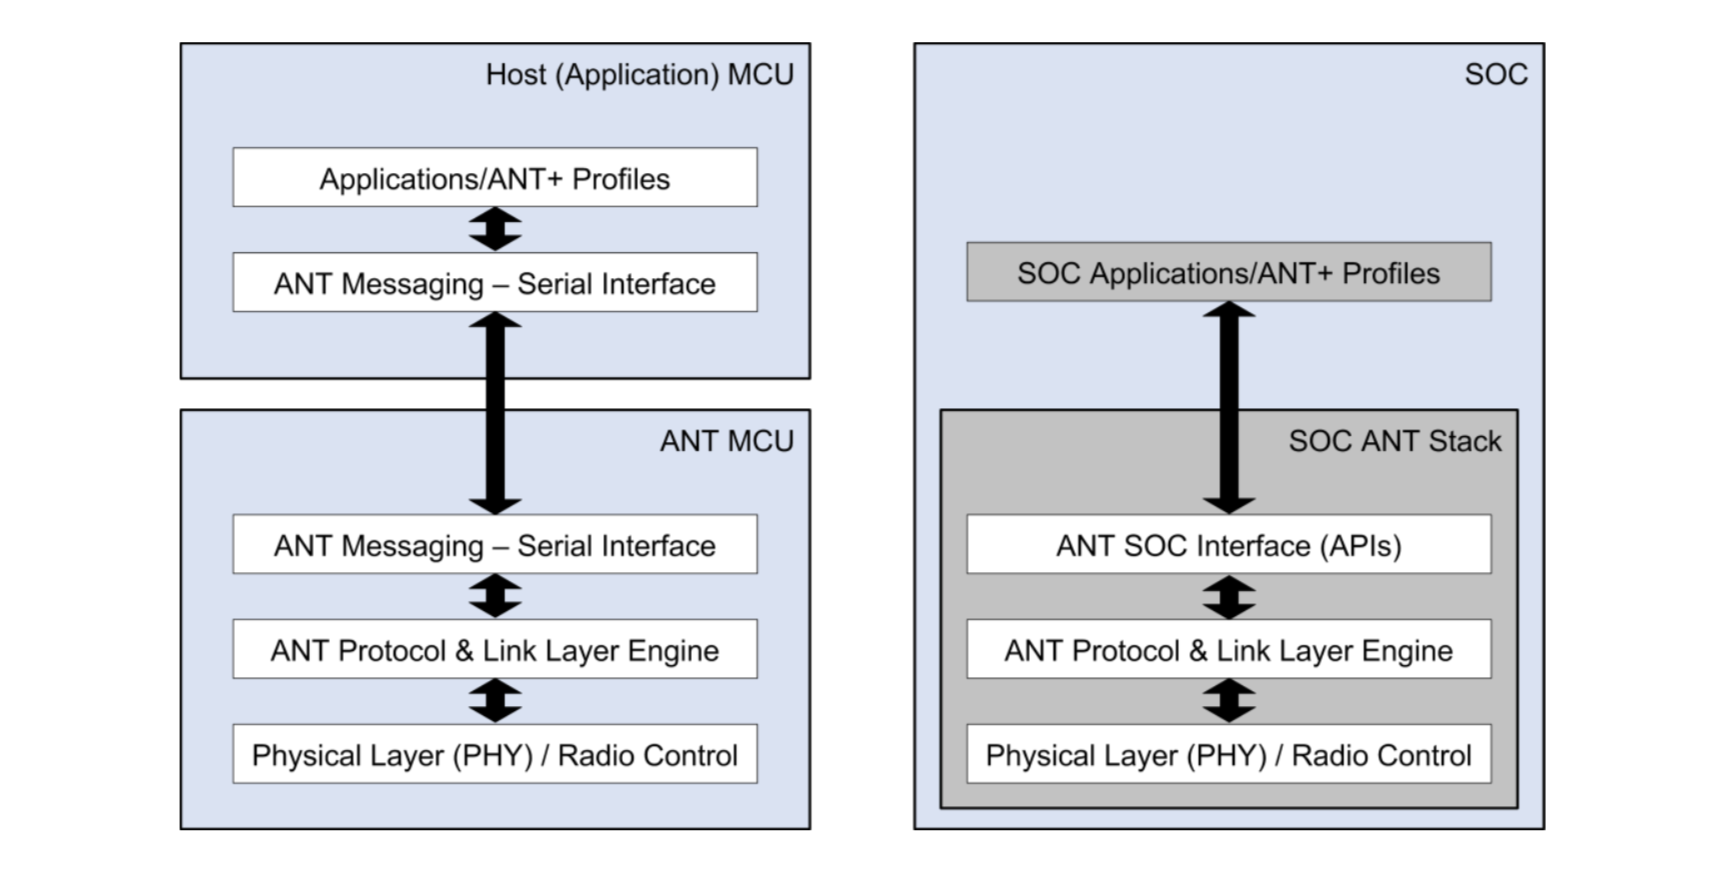
\includegraphics[width=0.5\columnwidth]{Figures/ANT_layers.png}
\caption{ANT layers}
\label{ANT_layers}
\end{center}
\end{figure}

\subsubsection{ANT base station}

The ANT base station is the slave which receives the broadcast messages. It establish multiple channels (in this project maximal 8 channels). Each channel is assigned to one radio frequency and one beacon's channel ID. This make sure itself listens to the broadcast of only one device. In this project, ANT base station is the ANT MCU (Figure / ref{ANT base station listening})`D52QD2M6IA` connected to host PC through USB interface board.  For more detail please refer to section 3.2. Steps to set up ANT communication.

 \textit{RSSI measuring in ANT base station} \\
 If "Extend Message" is enabled, ANT base station will provide its host application with additional information regarding the received data message. The additional information  includes received signal strength indication (RSSI)(shown in the figure \ref{ANT_base_station_configure}, step 8 receive messages). \\
 
Channel ID —— a 4 byte value that contains 3 fields: transmission type, device type  and device number.

\begin{itemize}
\item   Device Number
	\begin{itemize}
	\item  A 16-bit unique ID for ANT beacons.
	\item  The device numbers of ANT beacons are their serial numbers.
	\end{itemize}
\item Device Type
	\begin{itemize}
	\item To define the type (or class) of device.
	\end{itemize}
\item Transmission Type
	\begin{itemize}
	\item To define certain transmission characteristics of a device
	\end{itemize}
\item Radio frequency
	\begin{itemize}
	\item RF frequency value = (desire frequency - 2400MHz)/ 1MHz
	\end{itemize}
\end{itemize}

     
\subsubsection{ANT channels}

In this project we use synchronous, independent, bidirectional channels. In each ANT channel, only one master(transmitter) and one slave(receiver) is allowed. E.g. In the figure \ref{ANT_topology}, channel 1 is establish between beacon 1 and base station.

\begin{figure}[!h]
\begin{center}
\includegraphics[width=1\columnwidth]{Figures/ANT_base_station_diagram_configure.png}
\caption{ANT base station configure}
\label{ANT_base_station_configure}
\end{center}
\end{figure}

\begin{table}[!h]
\caption{Serial message format: ANT base station to Host PC}
\label{serial_message_format}
\begin{center}
\begin{tabular}{|l|l|l|l|l|}
\hline
Byte 1 & Byte 2 & Byte3 - N & Byte N + 1 & Byte N + 2 \\
\hline
Sync & Msg Length &  Msg ID & Message Content & Checksum \\
\hline
\end{tabular}
\end{center}
\end{table}

\begin{figure}[!h]
\begin{center}
\includegraphics[width=1\columnwidth]{Figures/ANT_base_station_diagram_listening.png}
\caption{ANT base station listening}
\label{ANT_base_station_listening}
\end{center}
\end{figure}


\begin{table}[!h]
\caption{Message format: ANT beacon to ANT base station}
\label{ANT_message_format}
\begin{center}
\small
\begin{tabular}{|p{2cm}|p{2cm}|p{2cm}|p{2cm}|p{2cm}|p{2cm}|p{2cm}|}
\hline
Byte 0 & Byte 1 & Byte 2 & Byte 3 & Byte4 & Byte 5 - 12 & Byte 13 \\
\hline
Sync  & Msg Length & Msg ID & Channel Number & Payload (serial number) &  Flag (0xC0) & Device Number \\
\hline
Byte 14 & Byte 15 & Byte 16 & Byte 17 & Byte 18 & Byte 19 & \\
\hline
Device Type & Transmission Type & Measurement Type & RSSI value & Threshold Configuration Value & Check sum & \\
\hline
\end{tabular}
\end{center}
\end{table}
\begin{figure}[!h]
\begin{center}
\includegraphics[width=1\columnwidth]{Figures/ANT_base_station_diagram_close_channel.png}
\caption{ANT base station close channel}
\label{ANT_base_station_close_channel}
\end{center}
\end{figure}

\subsubsection{Step 1: Implement GUI application for host PC}
\begin{enumerate}
\item Download ANT PC SDK 
\item Open ANT libraries solution in Microsoft Vitual Studio 2017.
\item  Build the solution and get library files `ANT\_LIB.lib`,`DSI\_SiUSBXp\_3\_1.dll`,`DSI\_SiUSBXp7\_3\_1.dll`.
\item Other library file: \url{C:\Program Files (x86)\Windows Kits\10\Lib\10.0.17134.0\um\x86\User32.Lib}
\item Implement an application on QT Using these library files. The structure of the application is shown in figure \ref{ANT_GUI_diaguram}.
\item Deploy the applicaion to a .exe file.
\end{enumerate}
To see how to use ANT GUI application, please refer to 3.2.5. Step 4: Measure the RSSI value.

\begin{figure}[!h]
\begin{center}
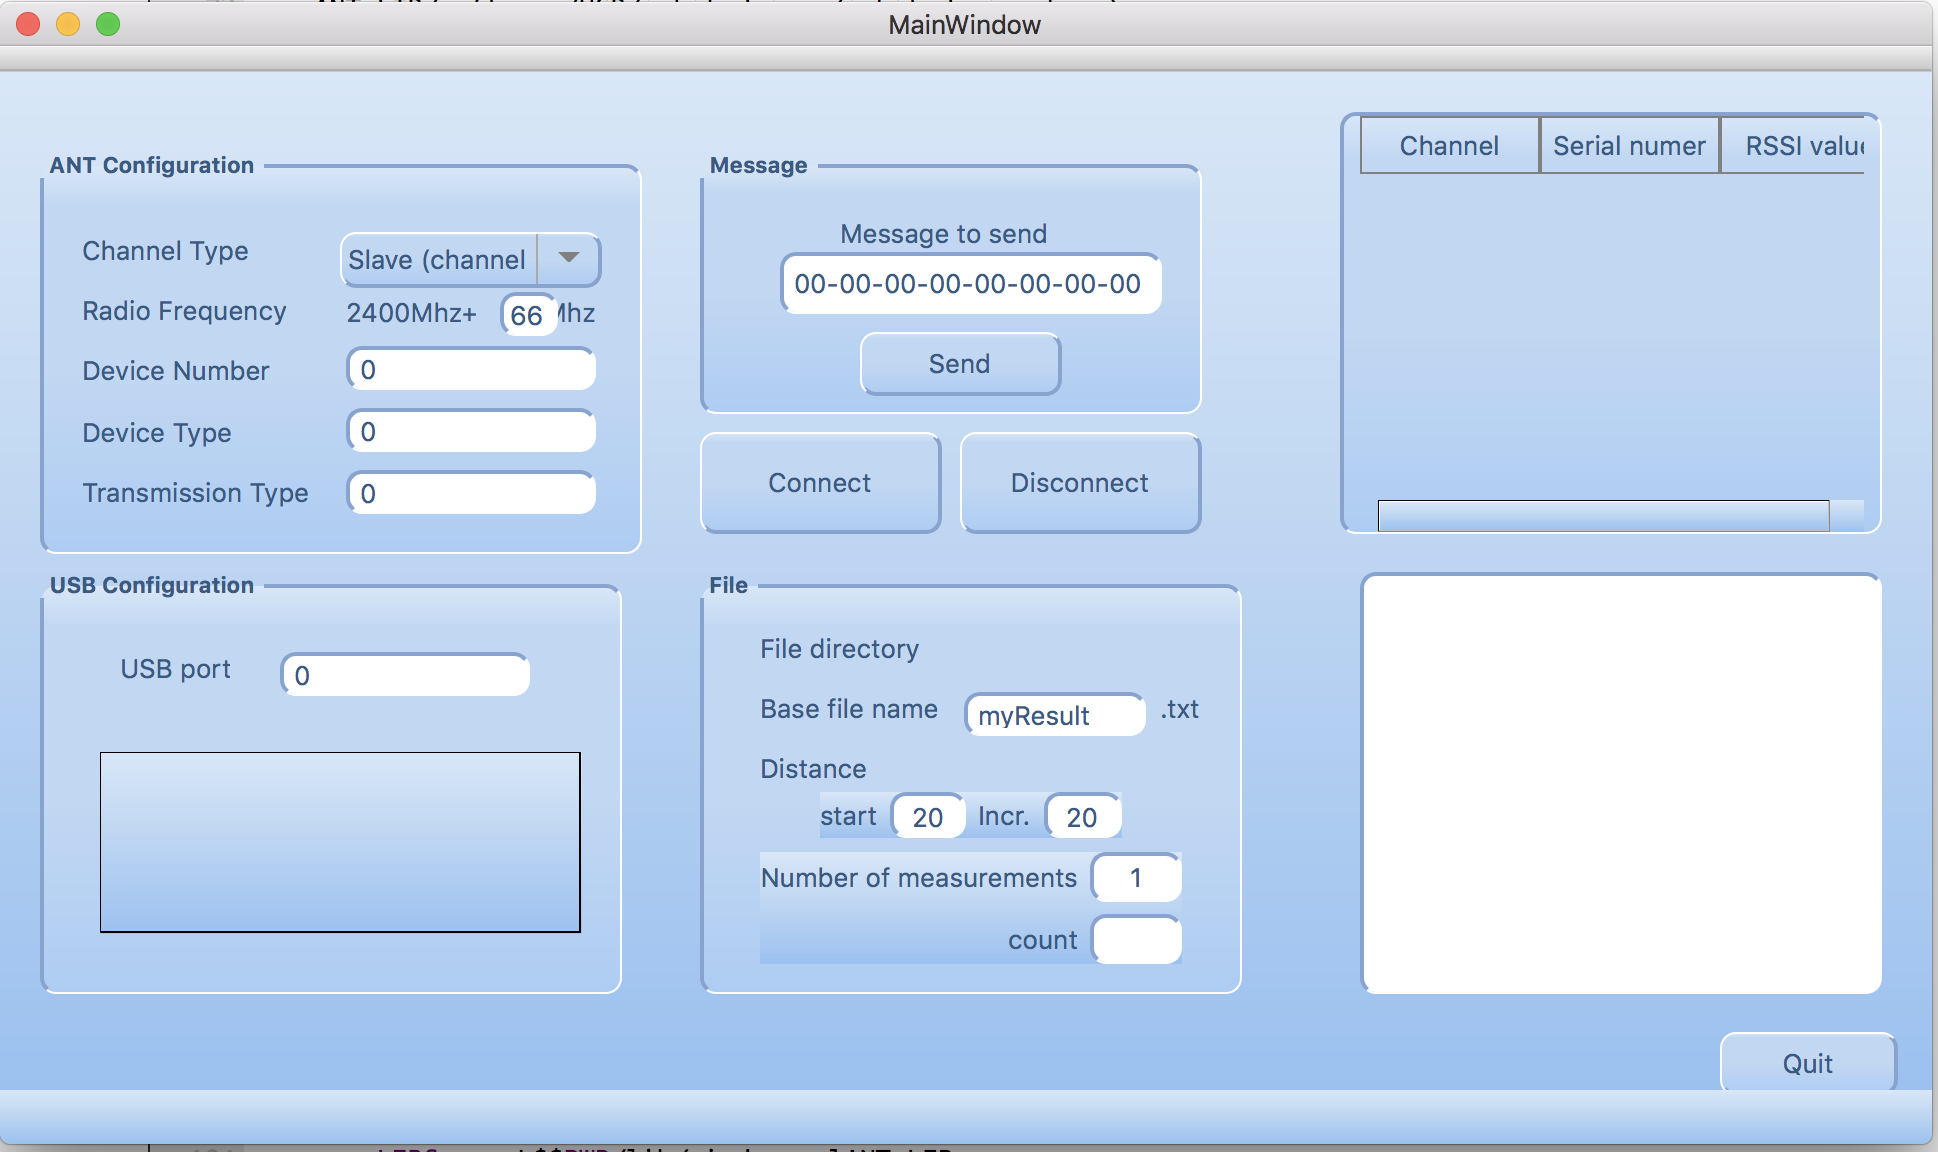
\includegraphics[width=1\columnwidth]{Figures/ANT_GUI_window.png}
\caption{ANT GUI window}
\label{ANT_GUI_window}
\end{center}
\end{figure}

\begin{figure}[!h]
\begin{center}
\includegraphics[width=0.7\columnwidth]{Figures/ANT_GUI_diaguram.png}
\caption{ANT GUI application structure}
\label{ANT_GUI_diaguram}
\end{center}
\end{figure}


\subsubsection{Step 2: Choose proper soft device for ANT beacons}
Please refer to IC revisions, SDK, and SoftDevice compatibility matrix for nRF52832. link: 
\url{http://infocenter.nordicsemi.com/index.jsp?topic=%2Fcom.nordic.infocenter.nrf52%2Fdita%2Fnrf52%2Fnrf52_comp_matrix.html} \\
To make sure the ANT and BLE application based on same soft device, we use SoftDevice S332 v5.0.0 and nRF5 SDK 14.2.0.

\subsubsection{Step 3: Implement application with SDK for ANT beacons}
The following step shows how to implement a ANT application using Keil. \\
\begin{enumerate}

\item Download NordicSemiconductor.nRF\_DeviceFamilyPack.8.17.0 and install it.

\item Connect a ANT SoC(D52QD2M6IA-A) to nRF 52 DK. And connect nRF52 DK to the host PC.

\item If any SDK is missing, SDK install window will automatically pop out. User can install all SDK packets for nRF52 DK.

\item Create a new project called ANT beacon project.

\item Go to Project menu, choose Option for Target... and configure you target as figure  \ref{Keil_configuration_1} and figure \ref{Keil_configuration_2}.

\item Write program for ANT beacon project according to the work flow (figure  \ref{ANT_beacon_workflow}) and compile it

\end{enumerate}

\begin{figure}[!h]
\begin{center}
\caption{Keil configuration 1}
\label{Keil_configuration_1}
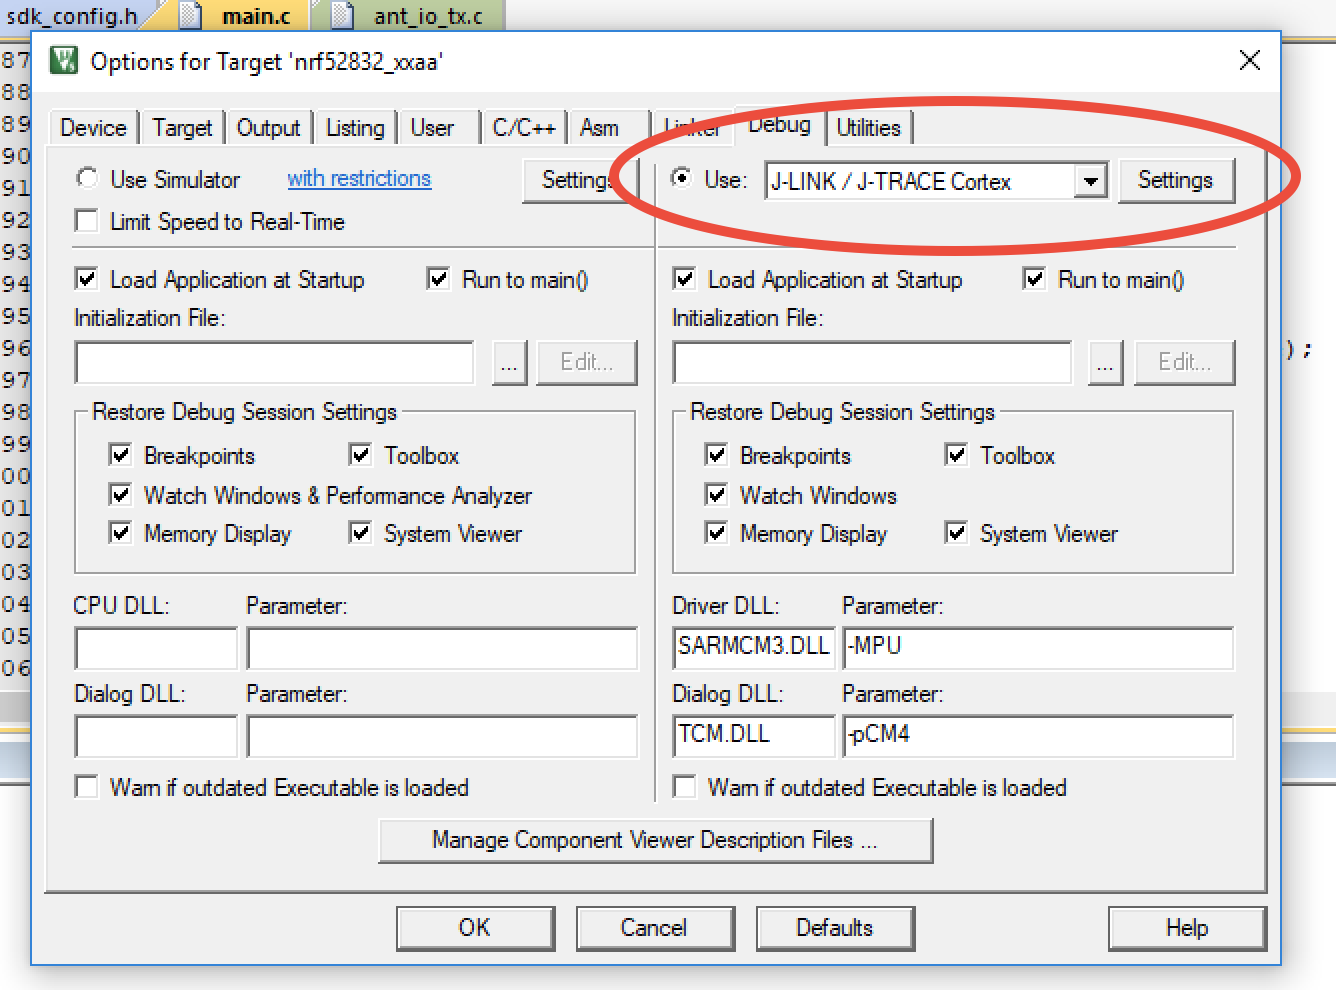
\includegraphics[width=0.5\columnwidth]{Figures/Keil_config_1.png}
\end{center}
\end{figure}

\begin{figure}[!h]
\begin{center}
\caption{Keil configuration 2}
\label{Keil_configuration_2}
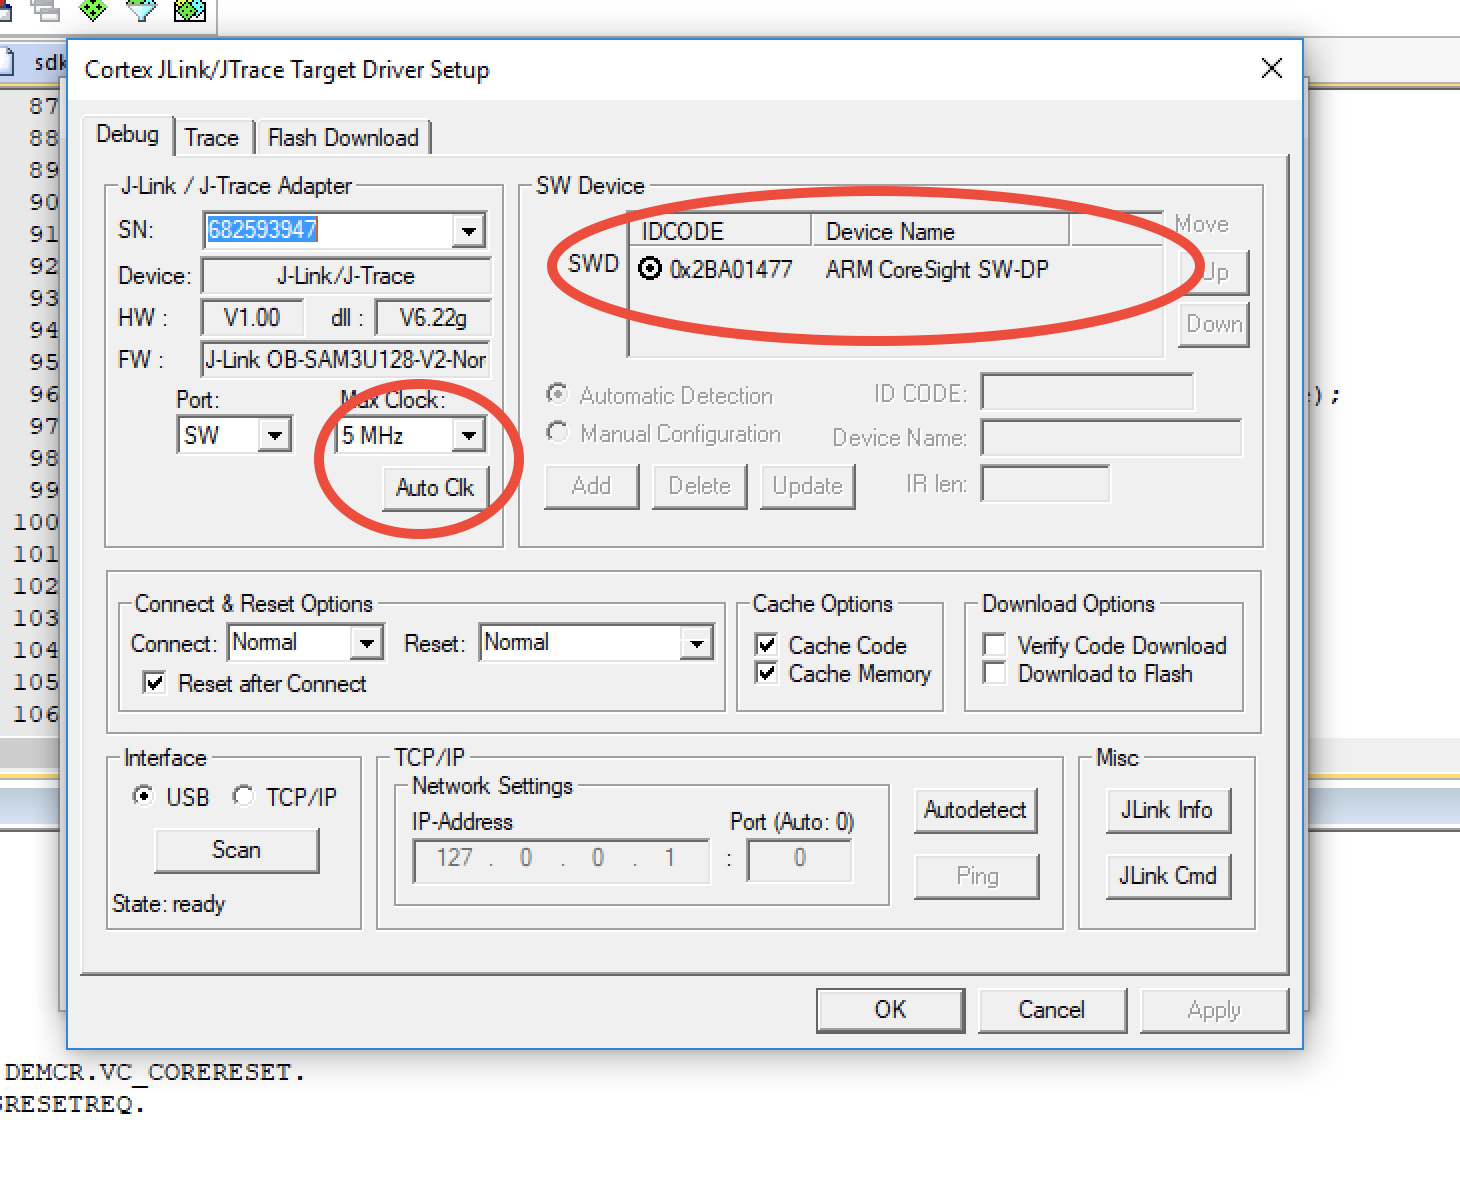
\includegraphics[width=0.5\columnwidth]{Figures/Keil_config_2.png}
\end{center}
\end{figure}

\begin{figure}[!h]
\begin{center}
\caption{ANT beacon workflow}
\label{ANT_beacon_workflow}
\includegraphics[width=0.5\columnwidth]{Figures/ANT_beacon_workflow.png}
\end{center}
\end{figure}

\subsubsection{Step 4: Measure the RSSI value}
The following step shows how to measure RSSI value for one ANT beacon in different distance. \\

\begin{enumerate}

\item Preparation on ANT beacons
	\begin{enumerate}
	\item  Connect a ANT SoC(D52QD2M6IA-A) to nRF 52 DK. And connect nRF52 DK to the host PC.
	\item  Open application "nRF studio" in host pc and flash  ANT\_s332\_nrf52\_5.0.0.hex(see download link in software list)  on the beacon(SoC).
	\item  Go to application tab and flash application .hex file( found in "\_build" folder 	of Keil project ) on the beacons.
		\begin{itemize}
		\item Another option: open Keil project and click "Load" icon to flash the ANT beacon project
		\end{itemize}
	\item Place an ANT beacon in desired start distance.
\end{enumerate}

\item Preparation on host PC
The following step shows how to Compiling and flashing the project onto the DK \\
	\begin{enumerate}
	\item Connect a ANT SoC "D52QD2M6IA" to nRF 52 DK. And connect nRF52 DK to the host PC.
	\item go to soft device tab and flash ANT soft device ANT\_s332\_nrf52\_5.0.0.hex on the ANT base station(SoC).
	\item Download Network Processor Source Code. Build this project and get  "ant\_network\_processor\_s332.hex".
	\item Open application "nRF studio" in host PC
	\item Go to application tab and flash application .hex file "ANT network proccessor S332"
The following step shows how set up GUI applicaion.
	\item Open ANT GUI application on the host PC
	\item Enter the configuration of the ANT beacons (Table 4). The channel type should be "Slave (channel 0 only)"
	\item Enter the base "file name" (e.g.myResult), "start distance" and "number of measurements".
	\end{enumerate}
	
\item Start  measuring
	\begin{enumerate}
	\item Turn on the ANT beacon.
	\item Click "Connect" bottom in GUI application.
	\item If an ANT base station is recognized, the VID and PID of the ANT base station will be shown in the text view. In addition, the received messages will be shown in Table view and text view. The "count"  value should be 1.  The measuring result will be stored in a txt file. 
		\begin{itemize}
		\item Txt file:  application path/file/base name\_start distance.txt
		\item E.g. application folder/file/myResult\_20.txt
		\end{itemize}
		
	\item Turn off the ANT ANT beacon. The base station will recognize its absence and the text view will print "RX Fail" and "Go to Search". if reach maximal number of measurement, the application will quit.  
	\item Move ANT beacon to next destance (start distance + Turn on the ANT beacon after "Go to search" is printed. The count value will puls 1. Now the measuring result will be store in a new txt tile. 
		\begin{itemize}
		\item New txt file: application path/file/base name\_start distance + increment.txt  
		\item E.g. application folder/file/myResult\_40.txt
		\end{itemize}
	\item Repeat step 5-6
	\end{enumerate}
\end{enumerate}

\begin{table}[!h]
\begin{center}
\caption{Default ANT GUI Application configuration for single channel base station}
\label{Default_ANT_GUI_config}
\begin{tabular}{|l|l|l|}
\hline
Parameter    & Value     & Description \\
\hline
Channel type  &  Slave ( multi channel)       & Each channel listens to  one beacon \\
\hline
 & Slave ( single channel) & to listen to one beacon \\
\hline
Device number  &  0  &  wildcard \\
\hline
Device Type    & 2 &  same as ANT beacon's device type \\
\hline
Transmission Type &  5 &  same as ANT beacon's transmission type \\ 
\hline
Radio frequency & 50 & desire frequency = 2450MHz \\
\hline
USB port & 0 & First USB device connected to PC \\
\hline
\end{tabular}
\end{center}
\end{table}

\subsection{BLE Setup}
The BLE topology is shown in figure \ref{BLE_topology}. the BLE beacons are broadcasters and the BLE base station is an observer. The observer listens to what's happening on the air. The broadcasters advertise but don't receive advertisement. They only use advertising but never establish a connection.
\begin{figure}
\begin{center}
\caption{BLE topology}
\label{BLE_topology}
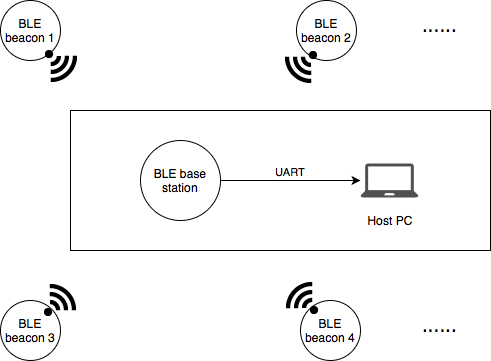
\includegraphics[width = 0.5\columnwidth]{Figures/BLE_topology.png}
\end{center}
\end{figure}

\subsubsection{BLE beacons}
The BLE beacons are broadcasters. they broadcasts its GAP name every time interval, known as the advertising interval. In this project, the BLE beacons are ANT SoC "D52QD2M6IA-A".

\begin{figure}
\begin{center}
\caption{BLE beacon diagram}
\label{BLE_beacon_diagram}
\includegraphics[width = 0.5\columnwidth]{Figures/BLE_beacon_diagram.png}
\end{center}
\end{figure}

\paragraph{GAP (Generic Access Profile): }
GAP is the lowest layer of the Bluetooth stack that an application interfaces with. It includes parameter that govern advertising and connection. e.g. name, address.

\subsubsection{Step 1: Implement application for BLE base staion}
The BLE base station is nrf52 DK. The application is implemented on Keil. The Keil project configuration is the same as ANT project (figure \ref{Keil_configuration_1} and figure \ref{Keil_configuration_2}). The workflow of application on BLE base station is shown in figure \ref{BLE_base_station_workflow}.

\begin{figure}
\begin{center}
\caption{BLE base station workflow}
\label{BLE_base_station_workflow}
\includegraphics[width = 0.5\columnwidth]{Figures/BLE_base_station_workflow.png}
\end{center}
\end{figure}

\subsubsection{Step 2: Implement application with SDK for BLE beacons} 
The BLEbeacon is SoC (D52QD2M6IA-A). The application is implemented on Keil. The Keil project configuration is the same as ANT project (figure 9 and figure 10). The workflow of applicaton on BLE beacon is shown in figure \ref{BLE_beacon_workflow}.

\begin{figure}
\begin{center}
\caption{BLE beacon workflow}
\label{BLE_beacon_workflow}
\includegraphics[width = 0.5\columnwidth]{Figures/BLE_beacon_workflow.png}
\end{center}
\end{figure}

\subsubsection{Step 3: Inplement application for host PC} 
\textit{this part is uncertain now because I may modify the application on host PC }
\subsubsection{Step 4: Measure the RSSI value}

The following step shows how to measure RSSI value for one BLE beacon in different distance.

\begin{enumerate}
\item Preparation on BLE beacon
	\begin{enumerate}
	\item Connect a ANT SoC(D52QD2M6IA-A) to nRF 52 DK. And connect nRF52 DK to the host PC. 
	\item Open application "nRF studio" in host pc and flash "ANT\_s33\_nrf52\_5.0.0.hex" on the beacon(SoC).
	\item Go to application tab and flash application .hex file( found in "\_build" folder of Keil project ) on the beacons.
		\begin{itemize}
		 \item another option: open Keil project and click "Load" icon to flash the BLE beacon
		\end{itemize}
   project
	\item Place an BLE beacon in desired start distance.

\end{enumerate}

\item Preparation on host PC

The following step shows how to Compiling and flashing the project onto the DK.

	\begin{enumerate}
	\item Connect nRF52 DK to the host PC.
	\item go to soft device tab and flash soft device "ANT\_s332\_nrf52\_5.0.0.hex" on the nRF52 DK.
	\item go to application tab and flash application .hex file( found in "\_build" folder of Keil project ) on the BLE beacons.
	\item another option: open Keil project and click "Load" icon to flash the BLE beacon project
	\end{enumerate}

\item Start measuring
\textit{this part is uncertain now because I may modify the application on host PC }
\end{enumerate}

\section{Evaluation}
\textit{Present the measurements in graphs and elaborate}

\section{Conclusions and Future Work}
\textit{Summarize your findings and elaborate on what else can be done}

\bibliographystyle{unsrt}
\bibliography{bibliography}

\section{Appendix}
The following software and hardware are used in the project:

\appendix
\section{Software}
\begin{itemize}
\item Mac OS 10.13

\item Virtualbox Windows 10 virtual machine

\item nRFgo Studio: a GUI applicaton for programming nRF5x SoftDevices, applications, and bootloaders. \\ Download here: \url{https://www.nordicsemi.com/eng/Products/Bluetooth-low-energy}

\item QT creater4.7 and QT  : a complete cross-platform development framework and IDE \\Dowload here:  \url{https://www.qt.io/download}

\item ANTware: an ANT Desktop applications used for testing, debugging and configuring \\ Download here: \url{ https://www.thisisant.com/developer/resources/downloads/#software_tab}

\item ARM Keil MDK 5: software develop solution for ARM based microcontrollers. 
\\Download here: \url{http://www2.keil.com/mdk5}

\item ANT USB Interface Board Driver - Windows 1.2.40.201: driver for the USB interface board in developer kit. \\ Download here: \url{https://www.thisisant.com/developer/resources/downloads/#software_tab}

\item Microsoft Visual Studio 2017 Full-featured IDE for Windows. \\Download here: \url{https://visualstudio.microsoft.com/downloads/}

\item Network Processor Source Code source code for ANT network processor firmware. it can build network processor firmwares for SoftDevices S212/S332, which is the application firmware for ANT base station. \\ Download here: 
\url{https://www.thisisant.com/developer/resources/downloads/}

\item soft device: ANT\_s332\_nrf52\_5.0.0.hex 
 BLE and ANT stack solution \\ Download here: \url{https://www.thisisant.com/developer/components/nrf52832#tab_protocol_stacks_tab}

\item nrf SDK 14: Source code of examples and libraries for application developing on SoC. \\Download here: \url{https://developer.nordicsemi.com/nRF5_SDK/nRF5_SDK_v14.x.x/}

\item ANT PC SDK  3.5: Source code of examples and libraries for Windows application developing. 

\item ANT Mac SDK 3.5: Source code of examples and libraries for Mac application developing. \\
Download ANT SDKs here: \url{https://www.thisisant.com/developer/resources/downloads/}

\item nRF5x MDK for Keil4:  nRF5x MDK for Keil4 and Keil5 compatibility version with 3-clause BSD license
https://www.nordicsemi.com/eng/Products/Bluetooth-low-energy/nRF52832

\end{itemize}
\section{Hardware}
\begin{itemize}
\item nRF52 DK: BLE base station 
\item ANT/BLE SoC Module: D52QD2M6IA-A: BLE and ANTbeacons
\item ANT SoC Module: D52QD2M6IA: ANT base station
\item ANTUIF1: USB interface board with a Molex socket: used to connect ANT base station with host PC.
\item ANTBAT3: Combined battery and I/O board with a Molex socket, a reset button, I/O. it is used to provide power for ANT beacons.
\item ANTUSB-M: ANT USB dongle
\end{itemize}


\end{document}
